Short peptides sit at a crossroads between liquid-like and solid-like self-assembly.
The same handful of residues that allow proteins to form liquid droplets inside cells
can also drive those proteins toward gels and amyloid fibrils.

In this thesis, we
stand at that crossroads and examine it through three lenses:

\begin{enumerate}
  \item the sequence rules behind liquid--liquid phase separation (LLPS) in
        intrinsically disordered proteins (IDPs) and their short sticker motifs,
  \item the energy landscape picture, which organizes all possible peptide
        conformations into a surface of minima and barriers, and
  \item a network perspective in which this landscape becomes a kinetic transition
        graph that can be analyzed with tools from Markov processes, spectral graph
        theory, and, more speculatively, statistical teleodynamics.
\end{enumerate}

This research is inherently interdisciplinary, drawing on condensate biology,
coarse-grained molecular simulation, Markov chain theory, spectral graph theory,
and statistical learning. Because the reader may enter with expertise in some of
these areas but not all, this chapter provides the necessary background across
each domain; each section builds toward the integrated framework deployed in the
Methods and Results chapters.

% Define pastel colors for the three thematic groupings
\definecolor{pastelblue}{RGB}{199,220,240}
\definecolor{pastelblueborder}{RGB}{120,160,200}
\definecolor{pastelgreen}{RGB}{200,230,201}
\definecolor{pastelgreenborder}{RGB}{120,180,130}
\definecolor{pastelorange}{RGB}{255,224,194}
\definecolor{pastelorangeborder}{RGB}{210,160,100}
\begin{figure}[ht]
\centering
\begin{tikzpicture}[
  % Section boxes: small, compact
  secbox/.style={
    rectangle, rounded corners=3pt, line width=0.6pt,
    minimum height=0.85cm, font=\footnotesize, align=center,
    text=black!80, inner sep=4pt
  },
  bluebox/.style={secbox, draw=pastelblueborder, fill=pastelblue, minimum width=3.6cm},
  greenbox/.style={secbox, draw=pastelgreenborder, fill=pastelgreen, minimum width=5.5cm},
  orangebox/.style={secbox, draw=pastelorangeborder, fill=pastelorange, minimum width=5.5cm},
  % Row labels
  rowlabel/.style={
    rectangle, rounded corners=5pt, line width=0.8pt,
    minimum height=1.0cm, font=\small\bfseries, align=center,
    text=black!70, inner sep=6pt, minimum width=12.8cm
  },
  bluelabel/.style={rowlabel, draw=pastelblueborder!60, fill=pastelblue!25},
  greenlabel/.style={rowlabel, draw=pastelgreenborder!60, fill=pastelgreen!25},
  orangelabel/.style={rowlabel, draw=pastelorangeborder!60, fill=pastelorange!25},
  % Arrows between rows
  rowarrow/.style={-{Stealth[length=4pt,width=4pt]}, thick, color=black!30},
]

% ===== Row 1: Physical systems (blue) =====
\node[bluelabel] (row1) {Physical Systems and Their Representation};

\node[bluebox, below=0.35cm of row1.south west, anchor=north west, xshift=0.15cm] (s1)
  {\textbf{\S\ref{sec:hexapeptides}}\\ IDPs, Condensates,\\[-1pt] and Sticker Motifs};
\node[bluebox, below=0.35cm of row1.south, anchor=north] (s2)
  {\textbf{\S\ref{sec:cg-models}}\\ Coarse-Grained\\[-1pt] Models};
\node[bluebox, below=0.35cm of row1.south east, anchor=north east, xshift=-0.15cm] (s3)
  {\textbf{\S\ref{sec:landscape-theory}}\\ Energy Landscapes\\[-1pt] and Disconnectivity};

% ===== Arrow: row 1 -> row 2 =====
\draw[rowarrow] ([yshift=-0.15cm]s2.south) -- ++(0,-0.7cm);

% ===== Row 2: Kinetic modelling (green) =====
\node[greenlabel, below=1.2cm of s2.south, anchor=north] (row2)
  {Kinetic Modelling and Network Analysis};

\node[greenbox, below=0.35cm of row2.south west, anchor=north west, xshift=0.65cm] (s4)
  {\textbf{\S\ref{sec:ktn}}\\ From Landscapes\\[-1pt] to Kinetic Models};
\node[greenbox, below=0.35cm of row2.south east, anchor=north east, xshift=-0.65cm] (s5)
  {\textbf{\S\ref{sec:graph-descriptors}}\\ Graph Theory, Spectral\\[-1pt] Methods, and Networks};

% ===== Arrow: row 2 -> row 3 =====
\coordinate (mid45) at ($(s4.south)!0.5!(s5.south)$);
\draw[rowarrow] ([yshift=-0.15cm]mid45) -- ++(0,-0.7cm);

% ===== Row 3: Prediction and interpretation (orange) =====
\node[orangelabel, below=1.2cm of mid45, anchor=north] (row3)
  {Prediction and Interpretation};

\node[orangebox, below=0.35cm of row3.south west, anchor=north west, xshift=0.65cm] (s6)
  {\textbf{\S\ref{sec:ml-lit}}\\ Statistical Learning\\[-1pt] for Prediction};
\node[orangebox, below=0.35cm of row3.south east, anchor=north east, xshift=-0.65cm] (s7)
  {\textbf{\S\ref{sec:stat_teleo_lit}}\\ Statistical\\[-1pt] Teleodynamics};

\end{tikzpicture}
\caption{Roadmap of the literature review. The seven sections are organized into
three tiers: the physical systems under study and how they are represented
computationally (\textcolor{pastelblueborder}{blue}), the kinetic models and
network-analysis tools built from those representations
(\textcolor{pastelgreenborder}{green}), and the statistical learning and
interpretive frameworks that connect network structure to kinetic behavior
(\textcolor{pastelorangeborder}{orange}). Each section provides essential background
for the integrated framework developed in the Methods chapter.}
\label{fig:lit-review-roadmap}
\end{figure}

Figure~\ref{fig:lit-review-roadmap} summarizes the progression: from the physical
systems and their coarse-grained representations, through kinetic models and
network analysis, to the statistical learning and interpretive frameworks that
connect structure to dynamics.


\section{Intrinsically Disordered Proteins, Condensates, and Sticker Motifs}\label{sec:hexapeptides}

\subsection{Biomolecular Condensates and Liquid--Liquid Phase Separation}

For most of the twentieth century, cellular organization was understood primarily
in terms of membrane-bound organelles, including the nucleus, mitochondria, the endoplasmic
reticulum, and so on. Over the past two decades, however, a parallel mode of
organization has come into focus. Cells also compartmentalize their biochemistry
using membraneless bodies that behave like liquid droplets. These structures fuse
on contact, relax into spherical shapes under surface tension, and exchange
molecules rapidly with the surrounding cytoplasm or nucleoplasm. Collectively,
they are known as \emph{biomolecular condensates}
\cite{Banani2017Review,Brangwynne2009,Hyman2014,Shin2017LLPS}.

The physical process that produces these droplets is liquid--liquid phase
separation (LLPS). In the simplest thermodynamic picture, a homogeneous solution
of macromolecules becomes unstable above a threshold concentration (or below a
threshold temperature), and the system separates into a dilute phase and a dense,
droplet phase. This physics can be analogized to the demixing of oil and water, but here the ``oil'' is a concentrated solution of proteins and nucleic acids, and the interactions that drive demixing are weak, multivalent, and often
sequence-specific \cite{Banani2017Review,Shin2017LLPS}.
Figure~\ref{fig:llps-schematic} illustrates this process schematically.

\begin{figure}[ht]
\centering
\begin{tikzpicture}[
  mol/.style={circle, fill=pastelblueborder, minimum size=3.5pt, inner sep=0pt},
  moldense/.style={circle, fill=pastelblueborder, minimum size=3.5pt, inner sep=0pt},
  box/.style={rectangle, rounded corners=4pt, draw=black!30, line width=0.6pt,
              minimum width=4.2cm, minimum height=3.8cm},
  phaselabel/.style={font=\scriptsize, text=black!60},
]

% --- Left panel: homogeneous solution ---
\node[box, fill=pastelblue!20] (homo) at (0,0) {};
\node[font=\small\bfseries, text=black!70, above=2pt of homo.north] {Homogeneous};

% Scatter molecules randomly but reproducibly
\foreach \x/\y in {
  -1.4/1.2, -0.7/0.9, 0.2/1.3, 1.0/0.8, 1.5/1.1,
  -1.2/0.3, -0.3/0.5, 0.6/0.1, 1.3/0.4, -0.9/-0.2,
  0.0/-0.1, 0.9/-0.4, -1.5/-0.5, -0.5/-0.7, 0.4/-0.9,
  1.2/-0.6, -1.0/-1.1, -0.1/-1.3, 0.7/-1.1, 1.5/-1.3,
  -1.4/-0.8, 0.3/0.7, -0.8/1.1, 1.1/-1.0, -0.2/0.0} {
  \node[mol] at (\x, \y) {};
}

% --- Arrow ---
\draw[-{Stealth[length=5pt,width=4pt]}, thick, black!40]
  (2.6,0) -- node[above, font=\scriptsize, text=black!50] {LLPS} (4.0,0);

% --- Right panel: phase-separated ---
\node[box, fill=pastelorange!15] (sep) at (6.8,0) {};
\node[font=\small\bfseries, text=black!70, above=2pt of sep.north] {Phase-separated};

% Dilute phase: sparse molecules
\foreach \x/\y in {
  5.3/1.2, 6.0/1.4, 8.0/1.0, 5.5/-1.2, 7.8/-1.1,
  8.2/0.3, 5.2/0.0, 8.1/-0.6, 5.6/0.7, 7.9/1.3} {
  \node[mol, fill=pastelblueborder!50] at (\x, \y) {};
}

% Dense droplet 1 (larger) -- no boundary drawn; condensate is membraneless
\foreach \x/\y in {
  6.3/0.5, 6.5/0.1, 6.7/0.6, 6.9/0.2, 6.4/0.3,
  6.8/0.5, 6.6/-0.1, 6.5/0.7, 6.7/0.0, 6.3/0.1,
  6.9/0.4, 6.6/0.4, 6.8/0.1, 6.4/0.6, 6.7/0.3,
  6.5/0.4, 6.8/-0.1, 6.6/0.2, 6.4/-0.1, 6.9/0.6} {
  \node[moldense] at (\x, \y) {};
}

% Dense droplet 2 (smaller) -- also no boundary
\foreach \x/\y in {
  7.2/-0.6, 7.4/-0.5, 7.6/-0.7, 7.3/-0.8, 7.5/-0.6,
  7.4/-0.9, 7.3/-0.5, 7.5/-0.8, 7.4/-0.7, 7.3/-0.7} {
  \node[moldense] at (\x, \y) {};
}

% Labels
\node[phaselabel] at (6.6,-1.6) {dense phase (no membrane)};
\node[phaselabel] at (8.0,0.6) {dilute};
\draw[-{Stealth[length=2.5pt,width=2pt]}, black!35, thin]
  (6.6,-1.4) -- (6.6,-0.5);

\end{tikzpicture}
\caption{Schematic of liquid--liquid phase separation. Left: a homogeneous
solution of macromolecules (blue dots) at uniform concentration. Right: above
a threshold concentration, the system spontaneously demixes into a dilute phase
and dense condensate droplets. Crucially, these condensates are
\emph{membraneless}: the boundary between the dense and dilute phases arises
solely from the thermodynamics of multivalent interactions, not from any
enclosing scaffold or membrane.}
\label{fig:llps-schematic}
\end{figure}

A striking feature of condensate-forming proteins is that many of them are
intrinsically disordered. Intrinsically disordered proteins (IDPs) and proteins
with long intrinsically disordered regions (IDRs) do not fold into a single
stable three-dimensional structure. Instead, they fluctuate among a large
ensemble of conformations, exposing interaction sites along the chain that can
transiently bind to partners. This conformational flexibility is not a defect.
It is purposefully designed for cells to tune phase behavior through modest changes in sequence, concentration, or post-translational modification
\cite{Boeynaems2018PhaseSep,Uversky2015IDPs}.


\subsection{Stickers, Spacers, and the Liquid-to-Solid Continuum}

A useful language for describing these systems is the \emph{stickers and spacers}
framework introduced by Choi, Holehouse, and Pappu \cite{Choi2020Stickers}.
In this picture, a disordered chain is divided into two functional classes of
residues. \emph{Stickers} are the residues or short motifs that mediate
attractive interactions: aromatic residues (tyrosine, phenylalanine, tryptophan)
that engage in $\pi$--$\pi$ stacking, cationic residues (arginine, lysine) that
participate in cation--$\pi$ contacts, and polar groups capable of specific
hydrogen bonding. \emph{Spacers} are the intervening residues that contribute
relatively little direct attraction but set the chain's flexibility, effective
reach, and solubility.

Within this framework, three design parameters control condensate behavior:

\begin{itemize}
  \item the \textbf{valence} of stickers, meaning how many sticky sites a single
        chain presents,
  \item the \textbf{patterning} of stickers along the chain, meaning whether they
        are clustered together or evenly distributed, and
  \item the \textbf{interaction strengths} of sticker--sticker contacts, which
        depend on the chemistry of the residues involved and on environmental
        conditions such as salt concentration, temperature, and pH.
\end{itemize}

Increasing the number of stickers or strengthening their interactions generally
lowers the saturation concentration at which LLPS occurs and can slow the
internal dynamics of the resulting droplets. Over time, some condensates
``mature'': their internal contacts become longer-lived and more directional,
and the droplet transitions from a liquid to a viscoelastic gel or even to a
solid aggregate rich in $\beta$-sheet structure. This liquid-to-solid continuum links LLPS directly to a broad class of
neurodegenerative and age-associated diseases, including amyotrophic lateral
sclerosis (ALS) and frontotemporal dementia, in which normally liquid condensates
harden into pathological aggregates \cite{Alberti2019Aging,Patel2015Nucleation}.

A schematic illustration of this ``beads-on-a-string'' view is shown in
Figure~\ref{fig:stickers-spacers-schematic}.

\vspace{3mm}
\begin{figure}[ht]
  \centering
  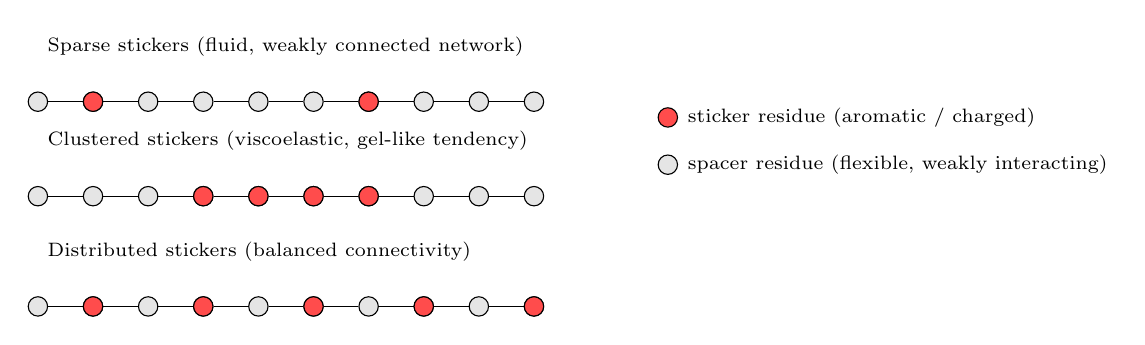
\begin{tikzpicture}[
      sticker/.style={circle, draw=black, fill=red!70, minimum size=7pt, inner sep=0pt},
      spacer/.style={circle, draw=black, fill=gray!20, minimum size=7pt, inner sep=0pt},
      chainlabel/.style={font=\scriptsize},
      >=stealth
    ]

    %-----------------------------
    % 1) Sparse stickers
    %-----------------------------
    \node[chainlabel, anchor=west] at (0,1.7)
      {Sparse stickers (fluid, weakly connected network)};
    \foreach \i in {0,...,9} {
      \node[spacer] (sparse-\i) at (\i*0.7,1) {};
    }
    % make a few of them stickers
    \foreach \i in {1,6} {
      \node[sticker] at (\i*0.7,1) {};
    }
    % bonds
    \foreach \i [evaluate=\i as \j using int(\i+1)] in {0,...,8} {
      \draw[-] (sparse-\i) -- (sparse-\j);
    }

    %-----------------------------
    % 2) Clustered stickers
    %-----------------------------
    \node[chainlabel, anchor=west] at (0,0.5)
      {Clustered stickers (viscoelastic, gel-like tendency)};
    \foreach \i in {0,...,9} {
      \node[spacer] (cluster-\i) at (\i*0.7,-0.2) {};
    }
    % cluster of stickers
    \foreach \i in {3,4,5,6} {
      \node[sticker] at (\i*0.7,-0.2) {};
    }
    % bonds
    \foreach \i [evaluate=\i as \j using int(\i+1)] in {0,...,8} {
      \draw[-] (cluster-\i) -- (cluster-\j);
    }

    %-----------------------------
    % 3) Distributed stickers
    %-----------------------------
    \node[chainlabel, anchor=west] at (0,-0.9)
      {Distributed stickers (balanced connectivity)};
    \foreach \i in {0,...,9} {
      \node[spacer] (dist-\i) at (\i*0.7,-1.6) {};
    }
    % evenly spaced stickers
    \foreach \i in {1,3,5,7,9} {
      \node[sticker] at (\i*0.7,-1.6) {};
    }
    % bonds
    \foreach \i [evaluate=\i as \j using int(\i+1)] in {0,...,8} {
      \draw[-] (dist-\i) -- (dist-\j);
    }

    %-----------------------------
    % Legend
    %-----------------------------
    \node[sticker,
          label=right:{\scriptsize sticker residue (aromatic / charged)}]
          at (8, 0.8) {};
    \node[spacer,
          label=right:{\scriptsize spacer residue (flexible, weakly interacting)}]
          at (8,.2) {};

  \end{tikzpicture}
  \caption{Schematic ``beads-on-a-string'' view of the stickers-and-spacers paradigm.
Red beads are attractive stickers and gray beads are inert spacers.
Top: sparse stickers yield a weak, fluid network.
Middle: clustered stickers promote locally dense, gel-like structures.
Bottom: distributed stickers support percolated yet dynamic networks.
The figure is not sequence-specific but illustrates how sticker patterning shapes
interaction networks relevant to LLPS and aging.}
  \label{fig:stickers-spacers-schematic}
\end{figure}


\subsection{Hexapeptides as Minimal Sticker Units}

While full-length IDRs can contain hundreds of residues, many of the key
interactions that drive LLPS and aggregation are encoded in short motifs. A
growing body of experimental and computational evidence shows that even very
short peptides can form ordered assemblies. Diphenylalanine (FF), for example,
self-assembles into nanotubes and fibrils \cite{Gazit2003}. Hexapeptides such as
\texttt{VQIVYK} (derived from the tau protein) and \texttt{NFGAIL} (derived from
islet amyloid polypeptide) are sufficient on their own to nucleate amyloid-like
$\beta$-sheet structures \cite{Eisenberg2005Hex}.

More recently, energy landscape studies have made this connection between short
motifs and self-assembly even more explicit. Roder and Wales analyzed
atomistic and coarse-grained energy landscapes for aggregation-prone peptide
fragments, finding that sequences with strong aggregation propensity tend to
exhibit multi-funnel landscapes with several deep, competing basins, while
control sequences show simpler, more directed funnels
\cite{Roder2018HexLandscapes}. Nicy and Wales extended this approach to
LLPS-relevant hexapeptides using a residue-level coarse-grained model,
directly connecting motif composition to both phase behavior and landscape
topology \cite{Nicy2024Mpipi,Wales2023PeptideTrees}.

Hexapeptides therefore serve as minimal but realistic ``sticker units'' for the
purposes of this thesis. They are small enough that large portions of their
conformational landscape can be sampled and analyzed computationally, but rich
enough to encode the sequence grammars that matter for LLPS and aggregation:
aromatic patterning, charge decoration, and polar ladders. This makes them an
ideal testbed for the landscape and network methods developed in the chapters
that follow.

In this thesis, the choice of hexapeptides over longer peptide sequences is deliberate.
Conformational space grows rapidly with chain length, and for longer peptides
the energy landscape becomes correspondingly more expensive to sample
thoroughly. At the hexapeptide scale, basin-hopping and discrete path sampling
can achieve near-exhaustive coverage of the stationary point database, producing
kinetic transition networks that faithfully represent the full landscape. This
completeness matters for the present study, because the graph-theoretic
descriptors we extract from the kinetic network are only meaningful if the
network itself is a reliable representation of the landscape rather than a
sparse, under-sampled sketch of it. Hexapeptides also retain enough sequence
diversity (aromatic content, charge patterning, polar contacts) to exhibit
genuinely complex, multi-funnel energy landscapes with real variation across
sequences. They, therefore, provide a controlled setting in which to develop and
validate the analysis framework before extending it to longer, more
biologically complete peptide systems.



\section{Coarse-Grained Models for Disordered Proteins}\label{sec:cg-models}

The previous section established that short peptide motifs, particularly hexapeptides, encode the essential sequence grammars that drive LLPS and aggregation. To study the conformational behavior of these peptides computationally, we need a molecular model that is both physically faithful and tractable enough to allow systematic exploration of energy landscapes across many sequences. This section reviews how coarse-grained models meet that need, and introduces the Mpipi model that provides the potential energy surface for all subsequent analysis in this thesis.

\subsection{Why Coarse-Grain?}

The most detailed computational approach to studying molecular behavior is
all-atom molecular dynamics with explicit solvent. In such simulations, every
atom of the protein and every surrounding water molecule is represented
individually, and the equations of motion are integrated at femtosecond
resolution. This level of detail captures local interactions with high fidelity,
but it comes at a steep computational cost. The timescales relevant for LLPS,
condensate maturation, and rare conformational transitions can span microseconds
to seconds, far beyond what routine all-atom simulations can reach for large
ensembles of sequences.

Coarse-grained (CG) models address this gap by simplifying the representation
of the molecule. In a typical residue-level CG model, each amino acid is
represented by a single interaction site (or ``bead''), and the solvent is
treated implicitly through effective pairwise potentials between beads. This
reduces the number of degrees of freedom by roughly two orders of magnitude
compared to an all-atom model and allows much longer timescales and larger
systems to be studied \cite{Dignon2020Review,Dignon2018HPS}.

Early CG models for IDPs focused on hydropathy (the tendency of each residue to
avoid or seek water) and generic electrostatic interactions. These models could
capture broad features such as chain expansion and collapse and could reproduce
some aspects of LLPS phase diagrams. However, they often underestimated the
importance of specific interaction types, particularly the aromatic and
cation--$\pi$ contacts that are now understood to be among the most important
sticker interactions in real condensate-forming proteins \cite{Das2020Comparative,Dignon2020Review,Dignon2018HPS,Regy2021ImprovedHPS,Vernon2018PiPi}.


\subsection{The Mpipi Model}

The Mpipi model, introduced by Joseph \emph{et al.} \cite{Joseph2021Mpipi},
was designed to address these limitations. It is a residue-level CG model in
which each amino acid is represented as a single bead, but the pairwise
interaction strengths between different residue types are parametrized with
particular care. The parameters are derived from a combination of atomistic
potentials of mean force (which capture the effective interaction between two
residues after averaging over solvent degrees of freedom) and experimental
benchmarks, with explicit tuning of aromatic--aromatic, cation--$\pi$, and
electrostatic interaction terms. The result is a model that can reproduce
single-chain dimensions (such as radii of gyration) and near-quantitative LLPS
phase diagrams for a range of disordered proteins.

Subsequent studies have confirmed that Mpipi and its variants capture subtle
sequence-level effects. These include shifts in critical temperature across
series of charge-patterning and aromatic-patterning mutants, as well as changes
in condensate viscosity that correlate with sticker composition
\cite{Nicy2024Mpipi,Cao2024CALVADOS}. For the hexapeptides studied in this
thesis, Nicy \emph{et al.} \cite{Nicy2024Mpipi} demonstrated that Mpipi
reproduces the thermodynamic trends observed in more detailed models and
experiments, and that it supports a controlled exploration of how sequence
grammar shapes both monomer and cluster landscapes.

From the perspective of this thesis, Mpipi plays a dual role. Practically, it
provides the potential energy function on which we define energy landscapes,
locate minima and transition states, and build kinetic models. Conceptually, it
grounds our analysis in a force field that has been calibrated against
LLPS-relevant experimental data. This means that patterns we find in the
landscapes and networks of Mpipi hexapeptides can be interpreted, at least
qualitatively, in terms of real sequence-dependent phase behavior, rather than
being artifacts of an arbitrary toy potential.


\section{Energy Landscapes and Disconnectivity Graphs}\label{sec:landscape-theory}

With a coarse-grained model in hand, we can define a potential energy surface for each hexapeptide sequence. But how do we make sense of a surface that lives in hundreds of dimensions and contains thousands of local minima? The energy landscape framework provides both the conceptual vocabulary and the computational tools for this task. This section reviews the theory of energy landscapes, introduces disconnectivity graphs as the standard visualization tool, and explains how landscape topology (funneled versus frustrated) relates to the kinetic behavior of molecular systems.

\subsection{The Energy Landscape Framework}

The idea that molecular behavior can be understood in terms of a potential
energy surface is one of the oldest and most powerful concepts in chemical
physics. For a system of $N$ atoms, the potential energy $V(\mathbf{x})$ is a
function of all $3N$ atomic coordinates (or, for a coarse-grained model, all
$3n$ bead coordinates, where $n$ is the number of beads). This function defines
a surface in a very high-dimensional space, and the behavior of the system can
be understood in terms of how it moves on this surface.

The key topological features of the surface are its \emph{local minima} and
its \emph{transition states}. Mathematically, both are stationary points where
the gradient vanishes, $\nabla V(\mathbf{x}) = \mathbf{0}$, but they differ in
the curvature of the surface at that point.

Let $\mathbf{H}(\mathbf{x})$
denote the Hessian matrix of second derivatives of $V$ evaluated at a
stationary point. A \emph{local minimum} is a stationary point at which all
eigenvalues of $\mathbf{H}$ are positive: the surface curves upward in every
direction, so any small displacement raises the energy. Such a point represents
a stable (or metastable) molecular structure. A \emph{transition state} (more
precisely, a first-order saddle point, or index-one saddle) is a stationary
point at which exactly one eigenvalue of $\mathbf{H}$ is negative and all
others are positive. The surface curves downward along one direction (the
reaction coordinate) and upward in all perpendicular directions. A transition
state, therefore, sits at the top of the lowest-energy ridge connecting two
adjacent minima, and the energy of the transition state relative to the minima
it connects defines the \emph{barrier height} for the transition between those
structures.

Energy landscape theory \cite{Onuchic1997NewView,Wolynes2004FoldingLandscape} reframes the folding problem in these terms. Folding is not a search along a single pathway.
Instead, it's biased diffusion on a high-dimensional surface that, for
evolutionarily selected proteins, has the shape of a \emph{funnel}. Although
the surface is rugged and contains many local minima, it is statistically
biased toward the native state, so that most trajectories eventually find their
way to the bottom. Wales placed the concept on rigorous mathematical footing \cite{Wales2003Book} and later developed computational tools for systematically
mapping the stationary points (minima and transition states) of molecular
energy landscapes and analyzing their global organization.

Two limiting cases illustrate the range of landscape architectures that arise
in practice. A \emph{funneled} landscape has one dominant basin that is much
deeper than any competitor, with relatively low barriers separating the many
local minima within that basin. Systems with funneled landscapes fold
efficiently and reach equilibrium quickly. A \emph{frustrated} or
\emph{multi-funnel} landscape, by contrast, has multiple deep basins of
comparable stability separated by high barriers. Such landscapes arise when
competing interactions (hydrophobic burial, hydrogen bonding, aromatic stacking)
stabilize qualitatively different structures. Systems with frustrated landscapes
can become kinetically trapped for long times, exhibiting slow relaxation,
hysteresis, and path-dependent behavior
\cite{Bryngelson1989SpinGlassProtein,Wales2003Book}. A schematic representation of this is in Figure \ref{fig:landscapes-three-regimes}.

\begin{figure}[H]
  \centering
  \includegraphics[width=0.8\textwidth]{./Figures/schematic_landscape}
  \caption{Schematic potential energy landscapes with increasing
  frustration. Left: a single, dominant funnel with one deep basin and only
  shallow alternatives, representative of compositionally simple or poly-X
  sequences. Middle: a broader funnel with one major competing basin and a
  shallower side basin, mimicking moderately frustrated sticker-based
  sequences. Right: a strongly branched, multi-funnel landscape with four
  near-degenerate basins separated by ridges, qualitatively similar to
  amyloid-prone sequences. Surfaces are shown as functions of two abstract
  collective variables $(CV_1,CV_2)$ and are intended as schematic
  illustrations rather than quantitative free-energy surfaces.}
  \label{fig:landscapes-three-regimes}
\end{figure}



\subsection{Disconnectivity Graphs}

Because the potential energy surface lives in hundreds or thousands of
dimensions, it cannot be visualized directly. Disconnectivity graphs, introduced
by Wales, Miller, and Walsh \cite{Wales1998Archetypal}, provide a compact, informative way to represent the hierarchical structure of such surfaces in a
single picture.

The construction is as follows. Each local minimum is represented by a vertical
line (a ``leaf'') whose lower endpoint sits at the energy of that minimum. As
one moves upward in energy, pairs of minima become mutually accessible when the
lowest barrier separating them falls below the current energy threshold. At
that energy, their branches merge. The process continues upward until all
branches have joined into a single tree. The resulting diagram looks like an
inverted tree, as represented by the schematic diagram in Figure \ref{fig:disconnectivity-schematic}: deep, narrow branches correspond to well-separated basins, while
broad, shallow branching indicates that many minima are easily interconvertible.

A landscape with a single dominant funnel produces a disconnectivity graph in
which most leaves feed into one deep central branch. A landscape with two or
more competing funnels produces a graph with multiple deep branches that remain
separate over a wide energy range. This visual signature makes disconnectivity
graphs a powerful diagnostic tool for classifying landscapes as funneled or
frustrated.

For peptide systems specifically, disconnectivity graphs have proven
particularly informative. Studies of amyloid-forming hexapeptides show that
strongly aggregation-prone sequences tend to produce tall, bushy trees with
several deep, nearly degenerate branches, while control sequences produce
narrower, more directed funnels \cite{Wales2023PeptideTrees,Roder2018HexLandscapes}.
More recent work on Mpipi hexapeptide clusters extended this picture, showing
how increasing the number of peptide copies in a cluster can either sharpen
funnels or amplify frustration, depending on the sequence composition
\cite{Nicy2024Mpipi}.


Because the full potential energy surface lives in hundreds of dimensions, we
never observe it directly. Disconnectivity graphs are the standard way to
collapse that complexity into a one-dimensional projection that preserves the
hierarchy of barriers without claiming to represent the literal geometry of the
surface. This makes them the natural, interpretable counterpart to the
schematic three-dimensional energy landscape figures shown in
Figure~\ref{fig:landscapes-three-regimes}, which serve only to build intuition
rather than to depict the actual geometry.
Figure~\ref{fig:disconnectivity-schematic} shows how the three landscape
regimes of Figure~\ref{fig:landscapes-three-regimes} translate into
disconnectivity graph topologies.

\begin{figure}[t]
  \centering
  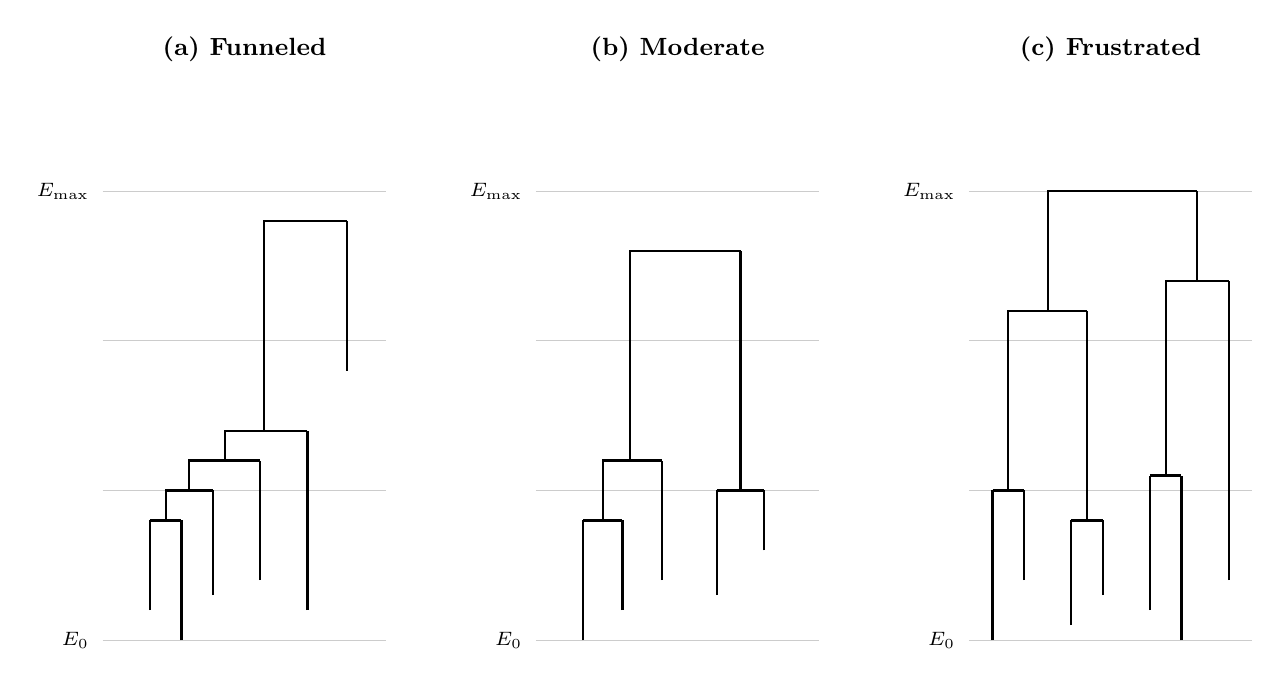
\begin{tikzpicture}[
      yscale=0.38,
      branch/.style={thick, draw=black},
      leaf/.style={thick, draw=black},
      elabel/.style={font=\scriptsize, anchor=east},
      title/.style={font=\small\bfseries, anchor=south},
    ]

    % -------------------------------------------------------
    %  (a) Funneled landscape
    % -------------------------------------------------------
    \begin{scope}[xshift=0cm]
      \node[title] at (1.5, 19) {(a) Funneled};
      % Energy ticks
      \foreach \e/\lab in {0/{$E_0$}, 5/{}, 10/{}, 15/{$E_{\max}$}} {
        \draw[gray!40] (-0.3, \e) -- (3.3, \e);
      }
      \node[elabel] at (-0.35, 0) {\scriptsize $E_0$};
      \node[elabel] at (-0.35, 15) {\scriptsize $E_{\max}$};

      % Deep main funnel: 5 leaves merging low
      \draw[leaf] (0.3, 1) -- (0.3, 4);
      \draw[leaf] (0.7, 0) -- (0.7, 4);
      \draw[branch] (0.3, 4) -- (0.5, 4) -- (0.7, 4);

      \draw[leaf] (1.1, 1.5) -- (1.1, 5);
      \draw[branch] (0.5, 4) -- (0.5, 5) -- (0.8, 5) -- (1.1, 5);

      \draw[leaf] (1.7, 2) -- (1.7, 6);
      \draw[branch] (0.8, 5) -- (0.8, 6) -- (1.25, 6) -- (1.7, 6);

      \draw[leaf] (2.3, 1) -- (2.3, 7);
      \draw[branch] (1.25, 6) -- (1.25, 7) -- (1.75, 7) -- (2.3, 7);

      % One shallow side minimum joining high
      \draw[leaf] (2.8, 9) -- (2.8, 14);
      \draw[branch] (1.75, 7) -- (1.75, 14) -- (2.3, 14) -- (2.8, 14);
    \end{scope}

    % -------------------------------------------------------
    %  (b) Moderately frustrated
    % -------------------------------------------------------
    \begin{scope}[xshift=5.5cm]
      \node[title] at (1.5, 19) {(b) Moderate};
      \foreach \e in {0, 5, 10, 15} {
        \draw[gray!40] (-0.3, \e) -- (3.3, \e);
      }
      \node[elabel] at (-0.35, 0) {\scriptsize $E_0$};
      \node[elabel] at (-0.35, 15) {\scriptsize $E_{\max}$};

      % Main funnel (left): 3 leaves
      \draw[leaf] (0.3, 0) -- (0.3, 4);
      \draw[leaf] (0.8, 1) -- (0.8, 4);
      \draw[branch] (0.3, 4) -- (0.55, 4) -- (0.8, 4);

      \draw[leaf] (1.3, 2) -- (1.3, 6);
      \draw[branch] (0.55, 4) -- (0.55, 6) -- (0.9, 6) -- (1.3, 6);

      % Competing funnel (right): 2 leaves
      \draw[leaf] (2.0, 1.5) -- (2.0, 5);
      \draw[leaf] (2.6, 3) -- (2.6, 5);
      \draw[branch] (2.0, 5) -- (2.3, 5) -- (2.6, 5);

      % Join the two funnels high
      \draw[branch] (0.9, 6) -- (0.9, 13) -- (1.6, 13) -- (2.3, 13);
      \draw[branch] (2.3, 5) -- (2.3, 13);
    \end{scope}

    % -------------------------------------------------------
    %  (c) Multi-funnel (frustrated)
    % -------------------------------------------------------
    \begin{scope}[xshift=11cm]
      \node[title] at (1.5, 19) {(c) Frustrated};
      \foreach \e in {0, 5, 10, 15} {
        \draw[gray!40] (-0.3, \e) -- (3.3, \e);
      }
      \node[elabel] at (-0.35, 0) {\scriptsize $E_0$};
      \node[elabel] at (-0.35, 15) {\scriptsize $E_{\max}$};

      % Funnel 1 (far left)
      \draw[leaf] (0.0, 0) -- (0.0, 5);
      \draw[leaf] (0.4, 2) -- (0.4, 5);
      \draw[branch] (0.0, 5) -- (0.2, 5) -- (0.4, 5);

      % Funnel 2
      \draw[leaf] (1.0, 0.5) -- (1.0, 4);
      \draw[leaf] (1.4, 1.5) -- (1.4, 4);
      \draw[branch] (1.0, 4) -- (1.2, 4) -- (1.4, 4);

      % Funnel 3
      \draw[leaf] (2.0, 1) -- (2.0, 5.5);
      \draw[leaf] (2.4, 0) -- (2.4, 5.5);
      \draw[branch] (2.0, 5.5) -- (2.2, 5.5) -- (2.4, 5.5);

      % Funnel 4
      \draw[leaf] (3.0, 2) -- (3.0, 6);

      % Merge 1+2 at 11
      \draw[branch] (0.2, 5) -- (0.2, 11) -- (0.7, 11) -- (1.2, 11);
      \draw[branch] (1.2, 4) -- (1.2, 11);

      % Merge 3+4 at 12
      \draw[branch] (2.2, 5.5) -- (2.2, 12) -- (2.6, 12) -- (3.0, 12);
      \draw[branch] (3.0, 6) -- (3.0, 12);

      % Merge everything at 15
      \draw[branch] (0.7, 11) -- (0.7, 15) -- (1.65, 15) -- (2.6, 15);
      \draw[branch] (2.6, 12) -- (2.6, 15);
    \end{scope}

  \end{tikzpicture}
  \caption{Schematic disconnectivity graphs corresponding to the three landscape
  regimes in Figure~\ref{fig:landscapes-three-regimes}. The vertical axis
  represents potential energy. Each vertical line (``leaf'') terminates at the
  energy of a local minimum; branches merge at the energy where the two basins
  they represent first become mutually accessible.
  (a)~A funneled landscape: most leaves merge into one deep central branch at
  low energy, with only a single shallow side minimum joining at high energy.
  (b)~Moderate frustration: two distinct branches (a main funnel and a competitor)
  persist over a wide energy range before merging near the top.
  (c)~A frustrated, multi-funnel landscape: four nearly degenerate branches
  remain separate until high energies, producing a tall, bushy tree with no
  single dominant funnel.}
  \label{fig:disconnectivity-schematic}
\end{figure}


It's worth noting that disconnectivity graphs can be constructed using either
potential energy or free energy on the vertical axis, and these two
representations need not have the same topology when entropic contributions
play a significant role \cite{Krivov2002FEDG,Wales2006PELvsFEL}. Free-energy
disconnectivity graphs incorporate basin volumes and temperature-dependent
entropic effects that can stabilize different regions of configuration space
than those favored by potential energy alone.

In this thesis, we work with
potential-energy disconnectivity graphs, which arise naturally from the
databases of stationary points produced by the landscape exploration software.
Although these graphs do not encode full free-energy information, they provide
a faithful and widely used structural summary of the underlying landscape organization,
including the distribution of minima, the hierarchy of barriers, funnel depth, the number and depth of competing basins, and the overall degree of frustration. These features are perfectly suited for the kinetic and
graph-theoretic analyses we pursue.


\section{From Landscapes to Kinetic Models}\label{sec:ktn}

Disconnectivity graphs and stationary-point databases tell us \emph{what} structures a peptide can adopt and \emph{how high} the barriers between them are. But they do not, on their own, tell us \emph{how fast} the system moves between these structures, or which transitions dominate the long-time dynamics. To answer these questions, we must convert the static landscape into a dynamical model. This section reviews the conceptual framework for that conversion and introduces the kinetic observables that serve as prediction targets throughout this thesis.

\subsection{From Energy Landscapes to Kinetic Transition Networks}

An energy landscape, on its own, describes the thermodynamic structure of a system, detailing which
structures are stable, how deep their basins are, and how high the barriers
between them rise. To understand the \emph{dynamics} of molecular processes such as LLPS and condensate maturation, one must go further and assign transition rates to the movements between minima. This is where the landscape becomes a kinetic model.

The conceptual framework for this transformation comes from \emph{discrete path sampling} (DPS), developed by Wales and extended in subsequent years \cite{Wales2002DPS}. The central idea is that the stationary points of the energy landscape (minima and transition states) can be systematically located using landscape exploration algorithms, and from these points, one can construct a network in which each minimum is a node and each transition state defines a directed edge between a pair of minima. Methods such as the doubly nudged elastic band \cite{Trygubenko2004DNEB} and hybrid eigenvector-following \cite{Munro1999HEF} make it possible to find transition states in a scalable way, even for moderately large systems.

Once the network of minima and transition states is in place, the dynamics can be captured using the framework of \emph{continuous-time Markov chains} (CTMCs) \cite{Wales2002DPS}. In a CTMC, each minimum becomes a state, and the rate of hopping from one state to a neighboring state is determined by transition state theory. This transforms the landscape into a weighted, directed graph where edges carry rate constants. The resulting kinetic transition network (KTN) fully specifies the dynamics: given an initial condition (a probability distribution over states), one can compute the time evolution of that distribution by solving the master equation for the network.

The distinction between kinetic transition networks built from landscape data and the Markov state models (MSMs) commonly used in the molecular dynamics community is worth noting \cite{Noe2013MSMReview,Pande2010MSMReview}. MSMs are constructed from long molecular dynamics trajectories: trajectory frames are clustered into discrete metastable states, and transition probabilities are estimated from observed transition counts between clusters. KTNs, by contrast, are constructed from a database of stationary points and do not require trajectory data; rates are computed from the barrier geometry and frequencies at each stationary point. Both approaches yield a Markov model, and both can be used to compute kinetic observables such as mean first-passage times (MFPTs) and relaxation timescales. However, the underlying data source and construction principle are fundamentally different.

\subsection{Graph Transformation and Coarse-Graining}

A practical challenge for KTNs is that even modestly sized molecules can have tens of thousands of local minima. Computing eigenvalues and MFPTs on such large, sparse matrices can be numerically delicate, especially when the quantities of interest depend on rare transitions involving extreme timescale separations.

Graph transformation (GT) provides an elegant solution to this problem \cite{Trygubenko2006GT,Stevenson2014GT,Wales2024FPT}. The core idea is to partition the states into two groups: a small set of ``kept'' states that are of direct interest (typically the minima belonging to the reactant and product basins, plus a few kinetically important intermediates) and a large set of ``intervening'' states that can be eliminated. The intervening states are then removed one by one from the network. At each removal step, the transition rates between the remaining states are updated (renormalized) in such a way that the kinetic quantities of interest between the kept states are preserved exactly.

This renormalization is particularly powerful because it preserves mean first-passage times: the reduced network containing only the kept states faithfully reproduces all MFPTs computed on the full microscopic network. This allows one to work with much smaller, more tractable models while retaining quantitative accuracy for the kinetic observables that matter. Recent work has demonstrated the robustness of GT-based coarse-graining on large networks with extreme timescale separations \cite{Stevenson2014GT,Wales2024FPT}.

In this thesis, the coarse-grained networks produced by graph transformation serve as the basis for all subsequent kinetic analysis. They allow us to compute MFPTs and relaxation times reliably, and they provide the reduced network on which we extract graph-theoretic descriptors (described in the next section). By working with validated, coarse-grained models, we ensure that any correlations we find between network structure and kinetics are not artifacts of incomplete or biased sampling.

\subsection{Kinetic Observables: MFPTs and Relaxation Times}

Two main kinetic quantities serve as targets for our analysis. The \emph{mean first-passage time} (MFPT) from one set of states to another is the average time for the system to make a transition between those sets starting from equilibrium within the first set. MFPTs between structurally or functionally distinct basins (e.g., a compact, folded-like state and an extended, aggregation-prone state) quantify the timescale of conformational rearrangements relevant to phase behavior and aggregation. The forward and backward MFPTs together characterize the asymmetry of the kinetics and the ease or difficulty of accessing one basin from another.

The second set of kinetic quantities are the \emph{relaxation times} of the system, which are determined by the eigenvalues of the generator matrix $Q$ of the CTMC. Because the columns of $Q$ sum to zero, zero is always an eigenvalue (corresponding to the stationary distribution). The non-zero eigenvalues define the relaxation timescales: the system asymptotically approaches the stationary distribution with time constants determined by these eigenvalues. The slowest relaxation time sets the overall timescale for equilibration. The ratio of the two slowest relaxation times reveals the dynamical structure: a large ratio indicates a single dominant slow process, while a ratio close to one indicates that multiple slow processes compete on similar timescales, which characterizes multi-funnel landscapes with several comparably high barriers.

These kinetic observables are the prediction targets throughout this thesis: we seek to understand whether the graph-theoretic structure of the network can anticipate or predict these quantities. The next section reviews the mathematical tools from graph theory and spectral analysis that provide the structural descriptors we will test as predictors.

\begin{figure}[ht]
  \centering
  \begin{tikzpicture}[
    block/.style={
      rectangle, rounded corners=3pt, draw=black!50, fill=black!8,
      line width=0.8pt, minimum width=3.2cm, minimum height=1.0cm,
      font=\small, align=center, text=black, inner sep=4pt
    },
    arrow/.style={-{Stealth[length=3pt,width=3pt]}, thick, color=black!50},
    annot/.style={font=\scriptsize\itshape, text=black!45},
  ]
    % Row 1
    \node[block] (landscape) at (0, 0) {Energy Landscape\\{\scriptsize minima + transition states}};
    \node[block] (ktn) at (5.5, 0) {Kinetic Transition\\Network (KTN)\\{\scriptsize nodes + weighted edges}};
    \node[block] (ctmc) at (11, 0) {Continuous-Time\\Markov Chain\\{\scriptsize generator $Q$, rates $k_{ij}$}};

    \draw[arrow] (landscape) -- (ktn) node[midway, above, annot] {DPS + TST};
    \draw[arrow] (ktn) -- (ctmc) node[midway, above, annot] {harmonic rates};

    % Row 2
    \node[block] (gt) at (2.75, -2) {Coarse-Grained\\Network\\{\scriptsize $Q^{\mathrm{eff}}$ on kept states}};
    \node[block] (obs) at (8.25, -2) {Kinetic Observables\\{\scriptsize MFPTs, relaxation times $t_k$}};

    \draw[arrow] (ctmc.south) -- ++(0,-0.5) -| (gt.north) node[pos=0.25, right, annot] {graph transformation};
    \draw[arrow] (gt) -- (obs) node[midway, above, annot] {spectral analysis};
  \end{tikzpicture}
  \caption{Conceptual flow from energy landscape to kinetic observables. Stationary points on the landscape are connected via discrete path sampling and assigned rates by harmonic transition state theory, yielding a kinetic transition network. The resulting continuous-time Markov chain is coarse-grained by graph transformation, and kinetic observables (MFPTs, relaxation times) are computed from the reduced generator.}
  \label{fig:landscape-to-observables}
\end{figure}


\section{Graph Theory, Spectral Methods, and Network Analysis}\label{sec:graph-descriptors}

The previous section established that a peptide's dynamics can be represented as a continuous-time Markov chain on a kinetic transition network. But having a network is not the same as understanding it. A KTN with thousands of nodes and edges encodes an enormous amount of information, and we need principled tools to compress that information into a manageable set of structural descriptors. This is where graph theory and spectral analysis enter the picture: they provide a mathematical language for quantifying how connected, how clustered, how bottlenecked, and how efficiently mixing a network is. These descriptors will later serve as the independent variables in our regression models for predicting kinetic observables.

\subsection{Graphs as Models of Complex Systems}

The use of graphs to model relational structure has a long history in
mathematics and the physical sciences, but the systematic application of
graph-theoretic and spectral tools to molecular systems is a more recent
development. In the context of this thesis, a kinetic transition network is,
mathematically, a weighted directed graph: each minimum is a node, each
transition is an edge, and the edges carry weights derived from rates, barrier
heights, or branching probabilities. Understanding what graph theory and
spectral analysis can tell us about such networks requires some background in
these fields.

\subsection{Spectral Graph Theory}

Spectral graph theory studies the relationship between the structure of a
graph and the eigenvalues of matrices associated with it, most commonly the
adjacency matrix, the graph Laplacian, or (for our purposes) the generator
matrix of a Markov chain defined on the graph. The foundational text by
Chung \cite{Chung1997SpectralGraph} established much of the modern framework,
showing how eigenvalues encode global structural properties such as
connectivity, expansion, diameter, and mixing time.

A key quantity in spectral graph theory is the \emph{algebraic connectivity},
introduced by Fiedler \cite{Fiedler1973Algebraic}, which is the second-smallest
eigenvalue of the graph Laplacian. This eigenvalue is zero if and only if the
graph is disconnected, and its magnitude measures how tightly connected the
graph is: a large algebraic connectivity implies that the graph cannot be
easily split into weakly connected components. For random walks and Markov
chains on graphs, the analogous quantity is the \emph{spectral gap} of the
transition matrix or generator, which determines the rate of convergence to
the stationary distribution. A large spectral gap implies fast mixing (the
system forgets its initial condition quickly), while a small spectral gap
implies slow mixing (there is a bottleneck that traps probability on one side
of the network for long times) \cite{Chung1997SpectralGraph}.

The connection between spectral properties and mixing rates has a precise
mathematical form. For a reversible Markov chain, the spectral gap of the
generator directly gives the slowest relaxation time of the system, and the
ratio of the two leading eigenvalues reveals whether the dynamics is dominated
by a single slow process or by several competing slow processes. These
relationships are not merely theoretical: they are the reason that spectral
descriptors are natural candidates for predicting kinetic observables in
molecular networks.

\subsection{Expander Graphs and the Ramanujan Bound}

A particularly elegant result from spectral graph theory is the theory of
\emph{expander graphs}, which are sparse graphs with strong connectivity
properties. The optimal expanders are \emph{Ramanujan graphs}, introduced by
Lubotzky, Phillips, and Sarnak \cite{Lubotzky1988Ramanujan}, which are
$d$-regular graphs whose nontrivial adjacency eigenvalues all lie within the
interval $[-2\sqrt{d-1},\, 2\sqrt{d-1}]$. Such graphs achieve near-optimal
expansion and logarithmic mixing times, meaning that random walks on them
converge to the stationary distribution as quickly as is theoretically
possible for a graph of that degree \cite{Murty2003RamanujanSurvey}.

Physical kinetic transition networks are neither regular nor unweighted, so
they cannot literally be Ramanujan graphs. However, the underlying principle
carries over: the closer a network's spectral properties come to the
theoretical bounds for its average degree, the better its connectivity and the
faster its mixing. In this thesis we compute a ``Ramanujan score'' that
quantifies how close a given KTN is to this theoretical ideal, using it as a
normalized indicator of network quality rather than a literal measure of
optimality.

\subsection{Shortest-Path Distances on Weighted Graphs}

Another classical family of graph-theoretic tools involves
\emph{shortest-path distances} on weighted graphs. Given a set of non-negative
edge weights, Dijkstra's algorithm computes the minimum total weight along any
path between two nodes. By choosing different edge-weight schemes, one can
probe different aspects of the network.

For molecular kinetic networks, natural choices of edge weight include barrier
heights (giving a measure of the minimum cumulative energy cost of traversing
the network between two basins), negative log-rates (giving a kinetically
weighted measure of distance that incorporates temperature and entropic
prefactors), and negative log-branching probabilities (giving a
probabilistic measure of how ``improbable'' the most likely path between two
points is). Each of these distance measures captures a different aspect of
the kinetic connectivity, and their asymmetries between forward and backward
directions reflect the directedness of the underlying Markov chain.

\subsection{Community Structure and Centrality}

Network science also provides tools for identifying mesoscale structure in
graphs. \emph{Community detection} algorithms seek partitions of the node set
into groups (``communities'' or ``modules'') that are more densely connected
internally than they are to one another
\cite{Newman2006Modularity}. When applied to kinetic
transition networks, communities correspond naturally to metastable basins:
groups of minima that interconvert rapidly among themselves but transition
slowly to other groups. The number, size distribution, and separation of
communities thus reflect the funnel structure of the energy landscape.

\emph{Centrality measures} identify which nodes or edges are most important
for maintaining connectivity. Betweenness centrality, for example, measures
how often a node lies on shortest paths between other pairs of nodes; high
betweenness identifies transition states or intermediates that serve as
obligatory waypoints for transitions between basins. In a kinetic network,
centrality measures can reveal whether the dynamics is funneled through a
small number of key bottleneck states or distributed broadly across many
alternative pathways.

\begin{figure}[ht]
  \centering
  \begin{tikzpicture}[
    catbox/.style={
      rectangle, rounded corners=3pt, draw=black!50, fill=black!8,
      line width=0.8pt, minimum width=3.6cm, minimum height=1.8cm,
      font=\small, align=center, text=black, inner sep=5pt
    },
    arrow/.style={-{Stealth[length=3pt,width=3pt]}, thick, color=black!50},
  ]

    \node[catbox] (spec) at (0, 0) {
      \textbf{Spectral}\\[2pt]
      {\scriptsize spectral gap $\gamma$}\\
      {\scriptsize gap ratio $|\lambda_2|/|\lambda_3|$}\\
      {\scriptsize spectral entropy}\\
      {\scriptsize Ramanujan score}
    };

    \node[catbox] (dist) at (4.5, 0) {
      \textbf{Distance-Based}\\[2pt]
      {\scriptsize barrier distances}\\
      {\scriptsize rate-based distances}\\
      {\scriptsize $-\ln k$ shortest paths}\\
      {\scriptsize directional asymmetries}
    };

    \node[catbox] (topo) at (9, 0) {
      \textbf{Topological}\\[2pt]
      {\scriptsize betweenness centrality}\\
      {\scriptsize closeness centrality}\\
      {\scriptsize community structure}\\
      {\scriptsize degree statistics}
    };

    % Central label
    \node[font=\small\bfseries, text=black!60] at (4.5, 1.8) {Families of Graph-Theoretic Descriptors};

    % Bottom: what they feed into
    \node[rectangle, rounded corners=3pt, draw=black!40, fill=black!4,
      line width=0.8pt, minimum width=11.5cm, minimum height=0.8cm,
      font=\small, align=center, text=black!60, inner sep=4pt]
      (target) at (4.5, -1.8) {Feature vectors for regression models
      (Sec.~\ref{sec:ml-lit}) $\longrightarrow$ predict $\log$ MFPT, $\log t_2$};

    \draw[arrow] (spec.south) -- ++(0,-0.4) -| ([xshift=-3cm]target.north);
    \draw[arrow] (dist.south) -- (target.north);
    \draw[arrow] (topo.south) -- ++(0,-0.4) -| ([xshift=3cm]target.north);

  \end{tikzpicture}
  \caption{Three families of graph-theoretic descriptors extracted from coarse-grained kinetic transition networks. Spectral descriptors capture mixing and relaxation properties, distance-based descriptors quantify the cost of traversing the network between basins, and topological descriptors characterize the mesoscale organization of the network. Together, these families form the feature set used in the regression analysis described in Section~\ref{sec:ml-lit}.}
  \label{fig:descriptor-families}
\end{figure}

Taken together, the spectral, distance-based, and topological descriptors reviewed in this section provide a comprehensive structural fingerprint of each kinetic transition network (Figure~\ref{fig:descriptor-families}). The question that remains is whether these structural fingerprints have genuine predictive power for kinetic observables. The next section reviews the statistical learning tools we use to answer that question.


\section{Statistical Learning for Structure-Property Prediction}\label{sec:ml-lit}

The graph-theoretic descriptors from the previous section provide a rich structural characterization of each kinetic transition network, but they are only useful if they bear a meaningful relationship to the kinetic quantities we care about. This section reviews the statistical learning tools that allow us to test that relationship rigorously: the QSAR/QSPR tradition in chemical engineering, the specific regression methods we employ, and the cross-validation strategy that guards against overfitting in the small-sample regime typical of molecular property prediction.

\subsection{The QSAR/QSPR Tradition}

The idea that molecular properties can be predicted from structural descriptors
has deep roots in chemical engineering and medicinal chemistry. Quantitative
structure-activity relationships (QSAR) and quantitative structure-property
relationships (QSPR) have been a staple of chemical informatics since the
1960s \cite{Cherkasov2014QSAR,Todeschini2000MolDescriptors}. The central
premise is straightforward: if one can compute a set of numerical descriptors
that capture the relevant structural features of a molecule (topological
indices, electronic properties, geometric descriptors), then a statistical
model trained on those descriptors can predict experimentally measured
properties such as binding affinity, solubility, toxicity, or reactivity.

This thesis applies essentially the same logic to a different kind of
structure-property relationship. Instead of predicting the biological activity
of a drug molecule from its chemical fingerprint, we predict the kinetic
behavior of a peptide system (MFPTs and relaxation times) from the structural
descriptors of its kinetic transition network (graph distances, spectral
properties, centrality, community structure). The ``structure'' is not the
molecular graph of covalent bonds, but the kinetic graph of conformational
transitions, and the ``property'' is not a thermodynamic observable but a
kinetic one. However, the underlying statistical learning framework is the
same.

\subsection{Linear Regression and Regularization}

The simplest tool in the regression toolkit is ordinary least squares (OLS),
which fits a linear model by minimizing the sum of squared residuals. OLS is
interpretable and well understood, but it can overfit when the number of
features is large relative to the number of observations, and it provides no
mechanism for feature selection.

Regularization addresses these limitations by adding a penalty term to the
objective function that discourages large coefficients. \emph{Ridge regression}
\cite{HoerlKennard1970Ridge} adds an $\ell_2$ penalty
($\lambda \sum_j \beta_j^2$), which shrinks all coefficients toward zero but
does not eliminate any features entirely. This stabilizes the fit and reduces
variance at the cost of introducing a small bias, a tradeoff that is
advantageous when features are correlated (multicollinear), as is often the
case with graph-theoretic descriptors.

The \emph{Lasso} (least absolute shrinkage and selection operator), introduced
by Tibshirani \cite{Tibshirani1996Lasso}, uses an $\ell_1$ penalty
($\lambda \sum_j |\beta_j|$). The geometry of the $\ell_1$ constraint promotes
sparsity: many coefficients are driven exactly to zero, so the Lasso
simultaneously performs regularization and feature selection. This is
particularly useful for identifying which among a large set of candidate
descriptors are genuinely predictive.

\emph{Elastic net} regression \cite{ZouHastie2005ElasticNet} combines the
$\ell_1$ and $\ell_2$ penalties, inheriting both the sparsity of the Lasso
and the stability of Ridge regression. The mixing parameter $\alpha$ controls
the balance between the two penalties, and the overall regularization strength
$\lambda$ is chosen by cross-validation. Elastic net is the default choice
when one suspects that groups of correlated features should be selected or
excluded together.

\subsection{Ensemble Methods}

When the relationship between descriptors and targets is nonlinear, tree-based
ensemble methods often outperform linear models. \emph{Random forests}
\cite{Breiman2001RandomForests} build many decision trees on bootstrapped
subsamples of the data, with each tree considering only a random subset of
features at each split. The predictions of the individual trees are then
averaged, which reduces variance and provides robustness to overfitting. Random
forests also yield a natural measure of feature importance based on how much
each feature reduces prediction error across the ensemble.

\emph{Gradient boosting machines} \cite{Friedman2001GBM} take a different
approach: rather than averaging independent trees, they build trees
sequentially, with each new tree trained to correct the residual errors of the
preceding ensemble. By fitting to the gradient of the loss function at each
step, gradient boosting can capture complex nonlinear relationships with high
accuracy, though it requires careful tuning of learning rate and tree depth to
avoid overfitting.

Both random forests and gradient boosting are widely used in QSAR/QSPR studies
and in materials informatics more broadly, where the number of descriptors can
be large and the underlying functional relationships are unknown a priori
\cite{Cherkasov2014QSAR}.

\subsection{Model Assessment and Cross-Validation}

A central challenge in regression modeling is assessing how well a fitted model
will generalize to new, unseen data. When the dataset is small (as is often the
case in molecular property prediction, where each data point corresponds to a
different molecule or, in our case, a different hexapeptide sequence), standard
train-test splits provide noisy estimates of predictive performance.

\emph{Leave-one-out cross-validation} (LOO-CV) provides a nearly unbiased
estimate of the generalization error in the small-sample regime
\cite{HastieTibshirani2009ESL}. In LOO-CV, one observation is held out at a
time, the model is trained on all remaining observations, and the held-out
observation is predicted. This cycle is repeated for every observation, and the
prediction errors are aggregated. The resulting estimate of test error uses
nearly all the available data for training at each step, making it suitable for
datasets with tens rather than hundreds of observations.

For feature importance and model interpretation, we use \emph{permutation
importance}: the decrease in predictive performance when the values of a single
feature are randomly shuffled. Features whose permutation causes a large
degradation in performance are deemed important; those whose permutation has
little effect are not. This approach is model-agnostic and can be applied
equally to linear and nonlinear models \cite{Breiman2001RandomForests}.

\begin{figure}[ht]
  \centering
  \begin{tikzpicture}[
    mbox/.style={
      rectangle, rounded corners=3pt, draw=black!50, fill=black!8,
      line width=0.8pt, minimum height=0.85cm,
      font=\small, align=center, text=black, inner sep=4pt
    },
    arrow/.style={-{Stealth[length=3pt,width=3pt]}, thick, color=black!50},
    annot/.style={font=\scriptsize\itshape, text=black!45},
  ]
    % Left column: linear methods
    \node[mbox, minimum width=3.2cm] (ols) at (0, 0) {OLS};
    \node[mbox, minimum width=3.2cm] (ridge) at (0, -1.0) {Ridge ($\ell_2$)};
    \node[mbox, minimum width=3.2cm] (lasso) at (0, -2.0) {Lasso ($\ell_1$)};
    \node[mbox, minimum width=3.2cm] (enet) at (0, -3.0) {ElasticNet ($\ell_1 + \ell_2$)};

    % Right column: ensemble methods
    \node[mbox, minimum width=3.2cm] (rf) at (5.5, -0.5) {Random Forest};
    \node[mbox, minimum width=3.2cm] (gb) at (5.5, -2.0) {Gradient Boosting};

    % Group labels
    \node[font=\small\bfseries, text=black!55] at (0, 1.0) {Linear Models};
    \node[font=\small\bfseries, text=black!55] at (5.5, 0.5) {Ensemble Models};

    % Annotations
    \node[annot, anchor=east] at (-2.0, 0) {interpretable};
    \node[annot, anchor=east] at (-2.0, -2.0) {sparse (feature selection)};
    \node[annot, anchor=west] at (7.6, -0.5) {nonlinear};
    \node[annot, anchor=west] at (7.6, -2.0) {sequential correction};

    % Bottom: LOO-CV
    \node[mbox, minimum width=10cm, draw=black!40, fill=black!4] (loocv) at (2.75, -4.5)
      {Leave-One-Out Cross-Validation (LOO-CV)\\
       {\scriptsize train on $M{-}1$ sequences, predict held-out sequence, repeat $M$ times}};

    % Arrows down
    \draw[arrow] (ols.south) -- ++(0,-0.2) -| ([xshift=-1cm]loocv.north);
    \draw[arrow] (enet.south) -- ([xshift=-1cm]loocv.north);
    \draw[arrow] (rf.south) -- ++(0,-0.9) -| ([xshift=1.5cm]loocv.north);
    \draw[arrow] (gb.south) -- ++(0,-0.2) -| ([xshift=1.5cm]loocv.north);

    % Output
    \node[mbox, minimum width=10cm] (output) at (2.75, -6.0)
      {RMSE, MAE on $\log$ MFPT and $\log t_2$ \quad + \quad feature importance rankings};
    \draw[arrow] (loocv) -- (output);

  \end{tikzpicture}
  \caption{Overview of the regression framework. Six model types spanning linear and ensemble methods are each evaluated using leave-one-out cross-validation on the hexapeptide dataset. Linear models (left) offer interpretability and, in the case of Lasso, automatic feature selection. Ensemble models (right) capture nonlinear relationships without explicit feature engineering. All models are assessed on the same held-out predictions, yielding comparable error metrics and feature importance rankings.}
  \label{fig:regression-overview}
\end{figure}

\subsection{Network Descriptors as ``Risk Factors'' for Kinetics}

The language of ``risk factors'' provides a useful analogy from quantitative
finance for how we use the descriptors described above. Factor models in
finance explain much of the variance in asset returns using a small number of
structural variables (market exposure, firm size, value). The individual
factors are not the returns themselves; they are compact structural summaries
that, taken together, predict returns.

We adopt the same logic here. Our ``returns'' are the logarithmic MFPTs and
relaxation times of the peptide system, and our ``factors'' are the graph
distances, spectral gaps, centrality measures, community statistics, and
sequence composition features computed from the kinetic network. By fitting
regression models with leave-one-out cross-validation, we test whether these
structural descriptors have genuine predictive power for kinetic observables.
When they do, this constitutes evidence that the structural organization of the
network carries useful, system-level information about the dynamics. When they
do not, it identifies limits of the network-based perspective.

The chemical engineering perspective is worth emphasizing here. Structure-property
prediction is one of the oldest and most productive themes in chemical
engineering, from group contribution methods for estimating thermodynamic
properties to modern machine learning for catalyst design and process
optimization \cite{Venkatasubramanian2003QSPR}. This thesis applies that same
tradition to a new domain: predicting kinetic properties of molecular systems
from the graph-theoretic structure of their energy landscape networks. The
descriptors are different (spectral gaps instead of topological indices, graph
distances instead of molecular fingerprints), but the underlying intellectual
framework, using structural information to predict behavior, is the same one
that has powered chemical engineering for decades.


\section{Statistical Teleodynamics as an Interpretive Lens}\label{sec:stat_teleo_lit}

The preceding sections have reviewed the tools for building kinetic models from energy landscapes and for extracting structural descriptors that may predict kinetic behavior. But even if these descriptors prove predictive, the question remains: \emph{why} should the structural organization of a network carry information about its dynamics? Statistical teleodynamics offers one possible answer to this question, framing it in terms of emergent organizational principles rather than microscopic mechanism.

\subsection{From Thermodynamics to Teleodynamics}

Classical statistical mechanics explains why equilibrium populations follow the Boltzmann distribution: among all possible distributions over microstates, the one that maximizes entropy subject to an energy constraint is the exponential distribution. This principle is extraordinarily powerful, but it speaks only about equilibrium populations, not about the pathways or flows by which systems reach equilibrium.

Statistical teleodynamics (ST), proposed by Venkatasubramanian \cite{Venkatasubramanian2017Teleodynamics}, extends this maximum-entropy logic to systems where emergent, purpose-like patterns appear at higher levels of organization. The central idea is that many complex systems settle into configurations that can be understood as maximizing a generalized notion of ``fairness'' or ``effective utility'' under constraints, with entropy reinterpreted as a measure of distributional fairness rather than physical disorder. The framework has been applied to a range of domains, from income distributions in economics to self-organization in chemical systems.

Crucially, ST does not replace thermodynamics; it generalizes the entropy-maximization principle to a broader class of systems and observables. In the same way that equilibrium populations follow from maximizing entropy over microstates, ST equilibria follow from maximizing fairness over pathways or options available to the system.

\subsection{Statistical Teleodynamics and Kinetic Transition Networks}

For landscape-based KTNs, the teleodynamic perspective suggests a specific question: can we infer something about the emergent kinetic organization of a peptide system by examining the structure of its network and the statistics of its flows, without computing explicit trajectory ensembles?

If we treat the different basins or routes through the landscape as ``options'' available to the system, then quantities such as MFPTs, path probabilities, and relaxation times encode how the system balances two competing pressures: \emph{accessibility} (favoring routes with low barriers and high rates) and \emph{diversity} (the existence of many alternative pathways). A system whose network structure distributes probability flux ``fairly'' among many accessible routes would, in the teleodynamic picture, be one that has reached a kind of organizational equilibrium.

In this thesis we adopt a cautious, operational stance toward this framework. We do not claim that peptides are optimizing anything in a literal sense. Molecules do not intend to fold, phase-separate, or choose one kinetic route over another. However, given the structure of their energy landscape, barrier topology, and allowable transitions, certain pathways attract probability flux more readily than others. Over many realizations, the system appears to ``choose'' patterns that reconcile energy, entropy, and structural constraints.

Our operational test is simple: we ask whether the graph-theoretic descriptors motivated by this network-level perspective (spectral gaps, distance asymmetries, connectivity measures) have predictive power for kinetic observables. When they do, we interpret this as evidence that the structural organization of the network carries meaningful information about the ensemble of possible trajectories. When they do not, we treat this as a negative result for the teleodynamic reading in the present, minimal setting. Either outcome is informative.


\section{Summary and Positioning of This Thesis}

The literature reviewed in this chapter provides the layered foundation on which this thesis is built. Each section has supplied a specific conceptual or technical ingredient, and together they define the intellectual context for the work that follows.

LLPS and the stickers-and-spacers framework establish that simple sequence grammars in disordered proteins, operating through aromatic, cation--$\pi$, and electrostatic interactions, are sufficient to drive phase separation, and that the same interactions can push condensates along a continuum from liquid to solid
\cite{Brangwynne2009,Banani2017Review,Patel2015Nucleation,Alberti2019Aging}.
Hexapeptides distill these grammars into a minimal, computationally tractable unit \cite{Gazit2003,Eisenberg2005Hex}.

Coarse-grained modeling, and the Mpipi model in particular, provides a
physically grounded potential energy surface on which landscapes can be defined,
sampled, and compared across sequences. Because Mpipi has been calibrated
against LLPS-relevant experimental data, patterns found in Mpipi landscapes
connect to real phase behavior rather than existing only within an abstract
model \cite{Joseph2021Mpipi,Nicy2024Mpipi}.

Energy landscape theory and disconnectivity graphs supply the conceptual
vocabulary (funnels, frustration, barrier hierarchies) and the visualization
tools needed to classify landscapes and relate their structure to kinetic
behavior \cite{Onuchic1997NewView,Wales2003Book,Wales1998Archetypal}.

Kinetic transition networks and graph transformation provide the machinery for
converting a landscape into a continuous-time Markov chain and then
coarse-graining that chain into a smaller, MFPT-faithful effective model on
which kinetic observables can be computed reliably
\cite{Wales2002DPS,Stevenson2014GT,Wales2024FPT}.

Graph-theoretic and spectral descriptors, informed by broader work on network
mixing and expander graphs, provide the structural ``risk factors'' that we
test as predictors of kinetics. Statistical teleodynamics offers a language for
interpreting any predictive power these factors exhibit, framing it in terms of
emergent organizational patterns rather than microscopic mechanism
\cite{Murty2003RamanujanSurvey,Venkatasubramanian2017Teleodynamics}.

What is missing from the existing literature, and what this thesis aims to
supply, is a focused, quantitative bridge between these layers. Specifically,
we seek to connect:

\begin{enumerate}
  \item the \textbf{energy landscapes} of Mpipi hexapeptides, as characterized
        by disconnectivity graphs and stationary point databases,
  \item the \textbf{structure of the associated kinetic transition networks},
        summarized by barrier-based distances, rate-based distances, spectral
        properties, centrality measures, and other graph descriptors computed
        on coarse-grained generators, and
  \item \textbf{LLPS-relevant kinetic observables}, specifically forward and
        backward MFPTs between reactant-like and product-like basins and the
        timescales of the slowest relaxation modes.
\end{enumerate}

Figure~\ref{fig:methodology-pipeline} summarizes the flow from biological
system to quantitative prediction as a single pipeline, showing how each
layer of background reviewed in this chapter feeds into the next.

\begin{figure}[htbp]
\centering
\begin{tikzpicture}[
  node distance=0.55cm and 0.0cm,
  stage/.style={
    rectangle, rounded corners=3pt, draw=black!50, fill=black!8,
    line width=0.8pt, minimum width=11.8cm, minimum height=1.15cm,
    font=\small, align=center, text=black
  },
  arrow/.style={-{Stealth[length=3pt,width=3pt]}, thick, color=black!50},
  lbl/.style={font=\scriptsize\itshape, text=black!60, anchor=west},
]
% --- Stage 1: Sequence ---
\node[stage] (seq)
  {Hexapeptide sequence library\\[-2pt]
   \scriptsize (e.g.\ VQIVYK, NFGAIL, FF, \ldots)};

% --- Stage 2: CG potential ---
\node[stage, below=of seq] (cg)
  {Coarse-grained potential energy surface\\[-2pt]
   \scriptsize Mpipi model: $V(\mathbf{r})$ with electrostatics,
   short-range, $\pi$--$\pi$ terms};

% --- Stage 3: Landscape sampling ---
\node[stage, below=of cg] (land)
  {Energy landscape exploration\\[-2pt]
   \scriptsize GMIN (basin-hopping $\to$ minima) \quad
   OPTIM (DNEB + hybrid eigenvector-following $\to$ transition states)};

% --- Stage 4: KTN ---
\node[stage, below=of land] (ktn)
  {Kinetic transition network (KTN)\\[-2pt]
   \scriptsize Nodes = local minima, \quad edges = transition states, \quad
   rates via harmonic TST};

% --- Stage 5: Microscopic CTMC ---
\node[stage, below=of ktn] (ctmc)
  {Microscopic CTMC via PyGT\\[-2pt]
   \scriptsize Generator $\mathbf{Q}$, branching matrix $\mathbf{B}$,
   stationary distribution $\boldsymbol{\pi}$};

% --- Stage 6: GT ---
\node[stage, below=of ctmc] (gt)
  {Graph transformation (GT) coarse-graining\\[-2pt]
   \scriptsize Remove high-energy / fast-escape nodes $\to$
   reduced $\widetilde{\mathbf{Q}}$ preserving MFPTs};

% --- Stage 7: Features ---
\node[stage, below=of gt] (feat)
  {Graph-theoretic feature extraction\\[-2pt]
   \scriptsize Barrier/rate/branching distances, spectral gap and ratio,
   Ramanujan score, centrality, communities};

% --- Stage 8: Regression ---
\node[stage, below=of feat] (reg)
  {Regression models with LOO-CV\\[-2pt]
   \scriptsize OLS, Ridge, Lasso, ElasticNet, Random Forest,
   Gradient Boosting $\to$ predicted $\log\,\overline{t}_{\mathrm{MFPT}}$};

% --- Arrows ---
\foreach \a/\b in {seq/cg, cg/land, land/ktn, ktn/ctmc, ctmc/gt, gt/feat, feat/reg}
  \draw[arrow] (\a) -- (\b);

% --- Side labels ---
\node[lbl, rotate=90, anchor=south] at ([xshift=-6.5cm]$(seq)!0.5!(cg)$)
  {Sec.~\ref{sec:hexapeptides}};
\node[lbl, rotate=90, anchor=south] at ([xshift=-6.5cm]$(cg)!0.5!(land)$)
  {Sec.~\ref{sec:cg-models}};
\node[lbl, rotate=90, anchor=south] at ([xshift=-6.5cm]$(land)!0.5!(ktn)$)
  {Sec.~\ref{sec:landscape-theory}};
\node[lbl, rotate=90, anchor=south] at ([xshift=-6.5cm]$(ktn)!0.5!(gt)$)
  {Sec.~\ref{sec:ktn}};
\node[lbl, rotate=90, anchor=south] at ([xshift=-6.5cm]$(gt)!0.5!(feat)$)
  {Sec.~\ref{sec:graph-descriptors}};
\node[lbl, rotate=90, anchor=south] at ([xshift=-6.5cm]$(feat)!0.5!(reg)$)
  {Secs.~\ref{sec:ml-lit},~\ref{sec:stat_teleo_lit}};

\end{tikzpicture}
\caption{Full analysis pipeline. Each row corresponds to a layer of the
  analysis, with section references on the left indicating where each component
  is introduced in this literature review. The pipeline begins with a
  hexapeptide sequence and terminates with regression-predicted kinetic
  observables, passing through coarse-grained modeling, landscape exploration,
  network construction, Markov chain formulation, graph transformation, and
  feature extraction. The Methods chapter describes the technical implementation
  of each layer in detail.}
\label{fig:methodology-pipeline}
\end{figure}

By constructing landscape-based KTNs for a family of hexapeptides,
coarse-graining them via MFPT-preserving graph transformation, extracting
graph-theoretic features from the reduced networks, and using those features as
explanatory variables in regression models for logarithmic MFPTs, we test, in a
controlled and minimal setting, whether the structural organization of a
kinetic network can anticipate the kinetic behavior that matters for condensate
physics. In doing so, we aim to show how ideas from energy landscapes, network
science, and statistical teleodynamics can be woven into a coherent,
quantitative picture of sequence-dependent peptide behavior.
